\documentclass[tikz,border=7pt]{standalone}
\usetikzlibrary{arrows}
\usetikzlibrary{arrows.meta}
\usetikzlibrary{calc} 
\tikzset{>=latex}

\begin{document}

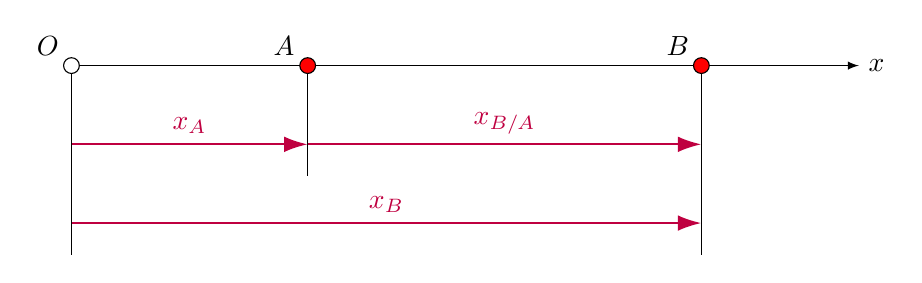
\begin{tikzpicture}
    % Define coordinates for the particles and vectors
    \coordinate (O) at (0,0);
    \coordinate (A) at (3,0);
    \coordinate (B) at (8,0);

    
    

    \draw[-{Latex[length=3mm,width=2mm]}, thick, purple] (0,-1) -- ($(A) + (0,-1)$) node[midway,above] {$x_{A}$};

    \draw[-{Latex[length=3mm,width=2mm]}, thick, purple] (0,-2) -- ($(B) + (0,-2)$) node[midway,above] {$x_{B}$};

    \draw[-{Latex[length=3mm,width=2mm]}, thick, purple] ($(A) + (0,-1)$)-- ($(B) + (0,-1)$) node[midway,above] {$x_{B/A}$};

    % Draw a frame of reference indicator
    \draw[->] (0,0) -- (10,0) node[right] {$x$};
    \draw[-] (0,0) -- (0,-2.4);
    \draw[-] (A) -- ($(A) + (0,-1.4)$);
    \draw[-] (B) -- ($(B) + (0,-2.4)$);
	
	% Draw the particles
	\filldraw[draw=black,fill=white] (O) circle [radius=1mm] node[left, above,xshift=-3mm] {$O$};
	\filldraw[draw=black,fill=red] (A) circle [radius=1mm] node[left, above,xshift=-3mm] {$A$};
	\filldraw[draw=black,fill=red] (B) circle [radius=1mm] node[left, above,xshift=-3mm] {$B$};


\end{tikzpicture}

\end{document}
